%----------------------------------------------------------------------------------------
%	SLIDE 3.
%----------------------------------------------------------------------------------------
\begin{frame}
\frametitle{Sample outputs of method I.}

\begin{figure}
	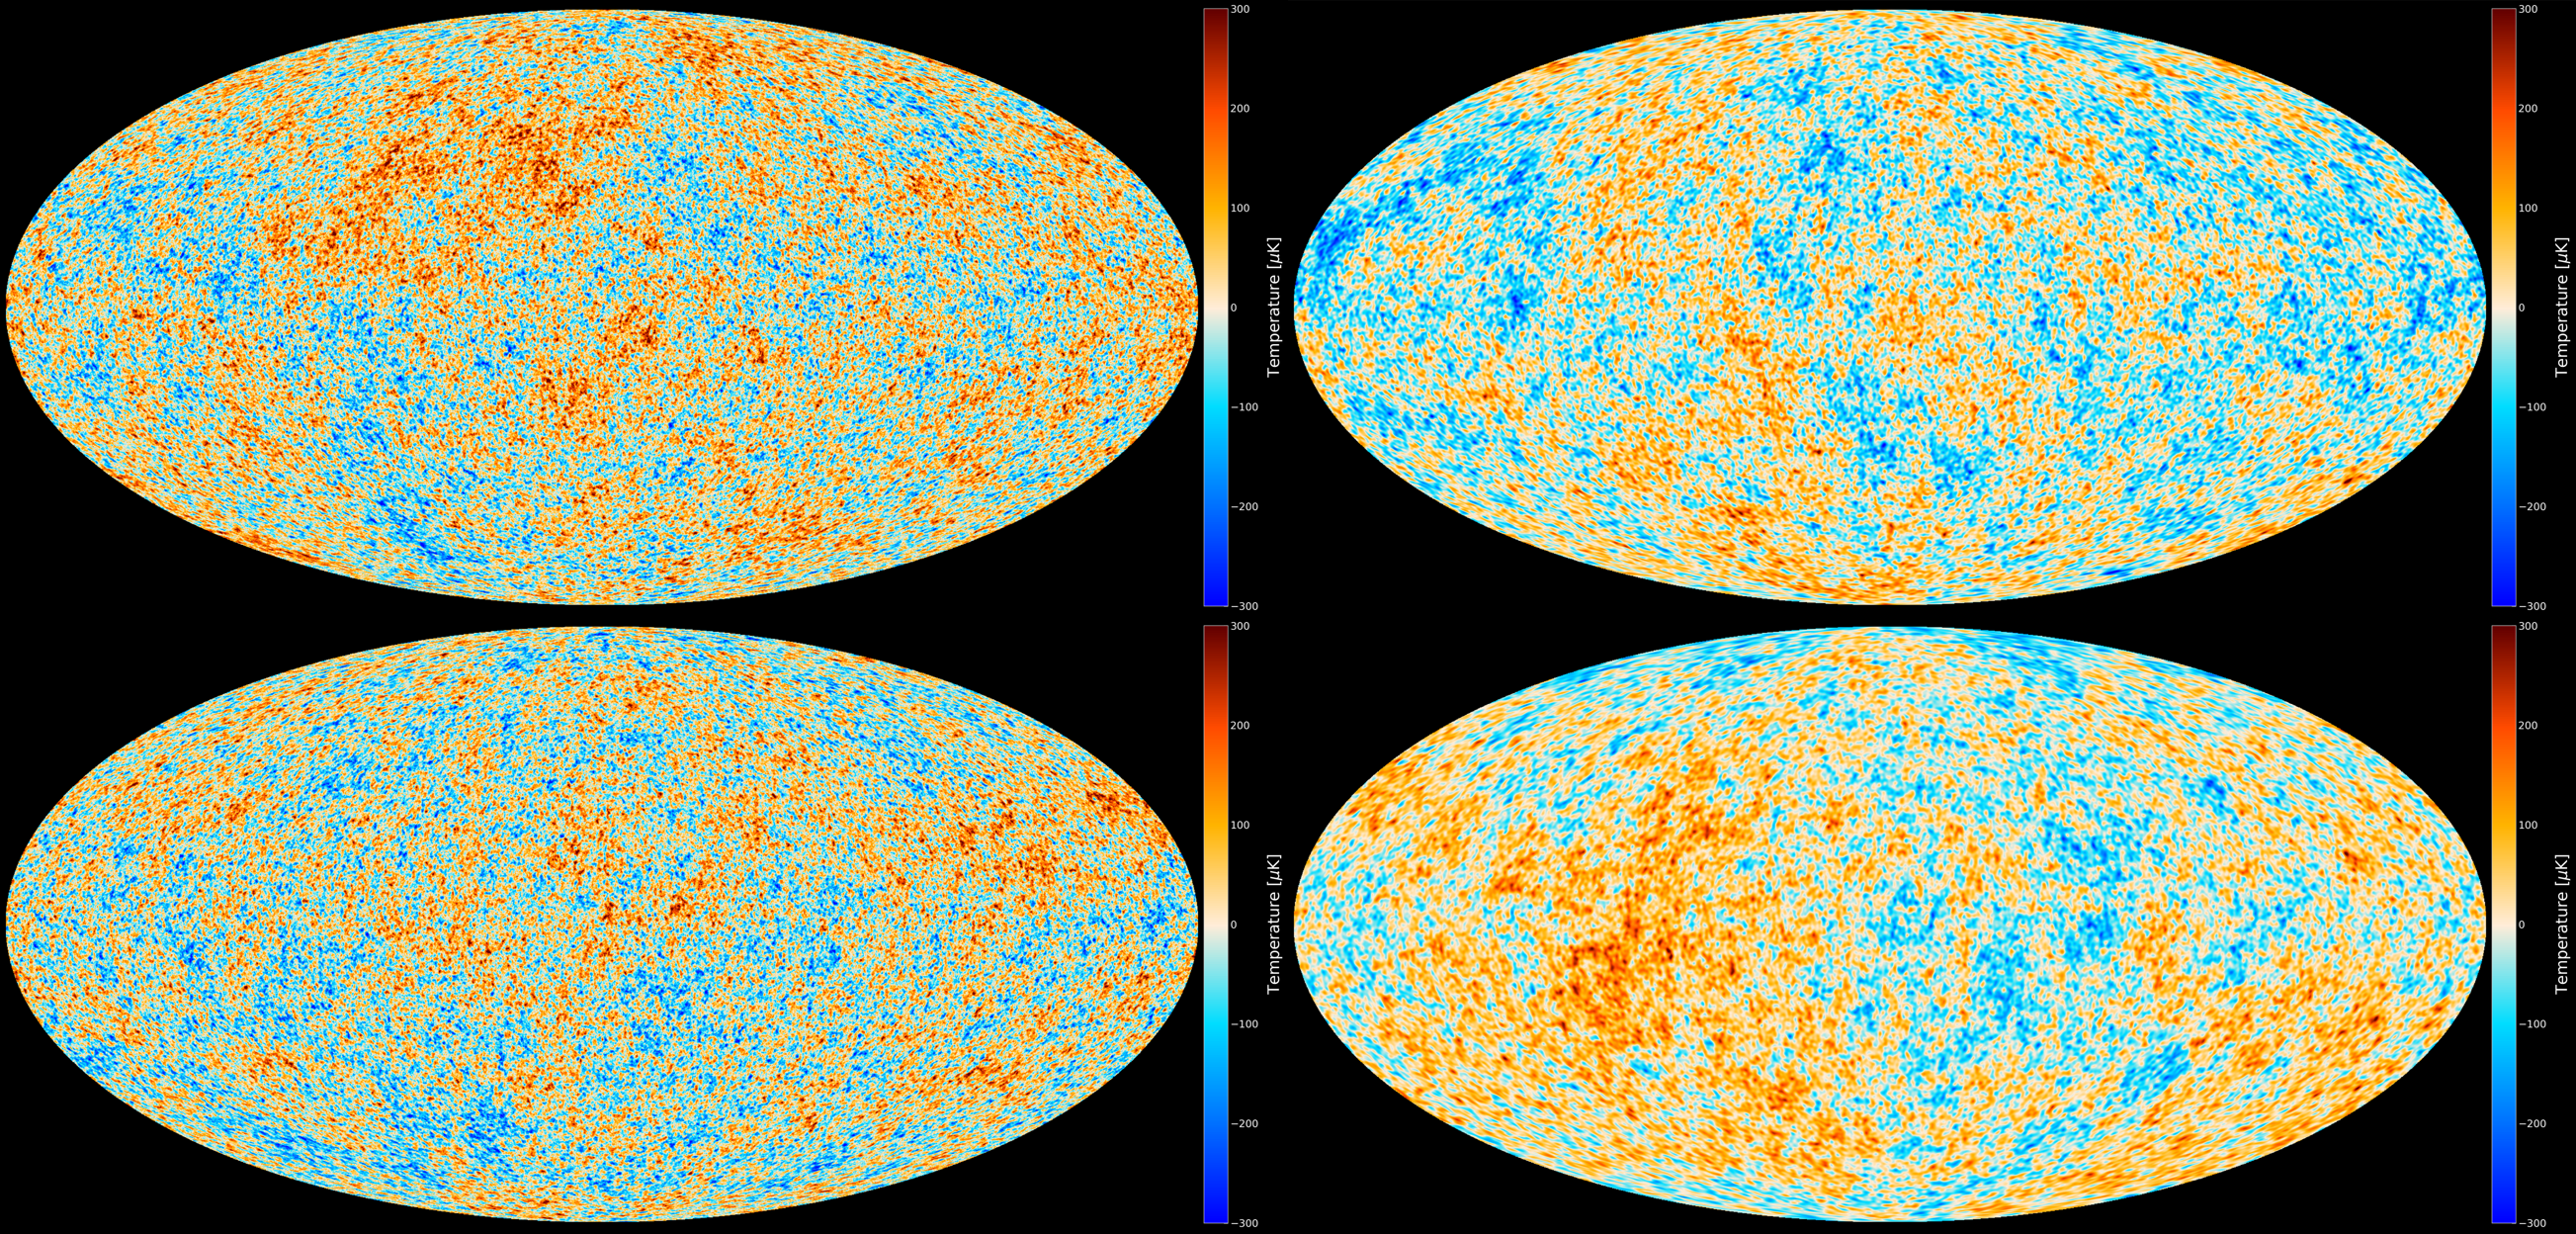
\includegraphics[width=\textwidth]{./images/CMB_HEALPix_sim_concat.png}
	\captionof{figure}{Randomly generated full-sky intensity maps of the CMB temperature anisotropy using HEALPix routines and conventions. The two images on the left side were generated with $\mathrm{FWHM}_{\mathrm{beam}} = 3\,\mathrm{arcmin}$ and with $\sigma_{\mathrm{beam}} = 0.5\,\mathrm{arcmin}$, while the images on the right side were generated with parameters $\mathrm{FWHM}_{\mathrm{beam}} = 30\,\mathrm{arcmin}$ and $\sigma_{\mathrm{beam}} = 15\,\mathrm{arcmin}$}
\end{figure}

\end{frame}